\documentclass[t,11pt,aspectratio=169]{beamer}
\usepackage{tikz}
\usepackage{pgfplots}
\usetikzlibrary{calc}
\usepackage[utf8]{inputenc}
\usepackage[ngerman]{babel}
\usepackage{amsmath,amsfonts,amssymb}
\usepackage{framed}
\usecolortheme{orchid}
\usepackage{etoolbox}
\useinnertheme[shadow=true]{rounded}

\usepackage{verbatim}

%%% PROGRESSBAR
\definecolor{pbblue}{HTML}{D8D8D8}% filling color for the progress bar
\definecolor{pbgray}{HTML}{F2F2F2}% background color for the progress bar
\useoutertheme{infolines}
\setbeamerfont{footline}{size=\normalsize}
\setbeamersize{text margin left=30pt,text margin right=30pt}
\makeatletter
\setbeamertemplate{footline}
{
	\leavevmode%
	\hbox{%
		\begin{beamercolorbox}[wd=.333333\paperwidth,ht=2.5ex,dp=1ex,center]{title in head/foot}%
			\usebeamerfont{title in head/foot}\insertshorttitle
		\end{beamercolorbox}%
		\begin{beamercolorbox}[wd=.333333\paperwidth,ht=2.5ex,dp=1ex,center]{date in head/foot}%
			%\usebeamerfont{date in head/foot}\insertshortdate{}\hspace*{2em}
			%\insertframenumber\hspace*{2ex} 
		\end{beamercolorbox}
		\begin{beamercolorbox}[wd=.333333\paperwidth,ht=3ex,dp=1ex,center]{author in head/foot}%
			\usebeamerfont{author in head/foot}\insertshortauthor~~%\beamer@ifempty{\insertshortinstitute}{}{(\insertshortinstitute)}
		\end{beamercolorbox}%
	}%
	\vskip0pt%
}
\makeatother
\makeatletter
\def\progressbar@progressbar{} % the progress bar
\newcount\progressbar@tmpcounta% auxiliary counter
\newcount\progressbar@tmpcountb% auxiliary counter
\newdimen\progressbar@pbht %progressbar height
\newdimen\progressbar@pbwd %progressbar width
\newdimen\progressbar@tmpdim % auxiliary dimension
\progressbar@pbwd=\linewidth
\progressbar@pbht=1.5ex
\def\progressbar@progressbar{%
    \progressbar@tmpcounta=\insertpagenumber
    \progressbar@tmpcountb=\insertdocumentendpage
    \progressbar@tmpdim=\progressbar@pbwd
    \multiply\progressbar@tmpdim by \progressbar@tmpcounta
    \divide\progressbar@tmpdim by \progressbar@tmpcountb
  \begin{tikzpicture}[rounded corners=3pt,very thin]
    \shade[top color=pbgray!20,bottom color=pbgray!20,middle color=pbgray!50]
      (0pt, 0pt) rectangle ++ (\progressbar@pbwd, \progressbar@pbht);
      \shade[draw=pbblue,top color=pbblue!50,bottom color=pbblue!50,middle color=pbblue] %
        (0pt, 0pt) rectangle ++ (\progressbar@tmpdim, \progressbar@pbht);
    \draw[color=normal text.fg!50]  
      (0pt, 0pt) rectangle (\progressbar@pbwd, \progressbar@pbht) 
        node[pos=0.5,color=normal text.fg] {\textnormal{%
             \pgfmathparse{\insertpagenumber*100/\insertdocumentendpage}%
             \pgfmathprintnumber[fixed,precision=0]{\pgfmathresult}\,\%%
        }%
    };
  \end{tikzpicture}%
}
\addtobeamertemplate{headline}{}
{%
  \begin{beamercolorbox}[wd=\paperwidth,ht=4ex,center,dp=1ex]{white}%
    \progressbar@progressbar%
  \end{beamercolorbox}%
}
\makeatother

\setbeamertemplate{frametitle}[default][center]

%%% BLOCKS
% block = Aufgabe
\setbeamercolor{block title}{fg=black,bg=blue!30!white} 
\setbeamercolor{block body}{fg=black, bg=blue!3!white}

% alertblock = Definition
\setbeamercolor{block title alerted}{fg=black,bg=red!50!white} 
\setbeamercolor{block body alerted}{fg=black, bg=red!3!white}

% exampleblock = Wiederholung
\setbeamercolor{block title example}{fg=black,bg=green!30!white} 
\setbeamercolor{block body example}{fg=black, bg=green!3!white}

\setbeamercovered{transparent}
\setbeamertemplate{navigation symbols}{}

\addtocounter{page}{-1}
\addtocounter{framenumber}{-1}
\setbeamercovered{invisible}





\pgfmathdeclarefunction{gauss}{2}{\pgfmathparse{1/(#2*sqrt(2*pi))*exp(-((x-#1)^2)/(2*#2^2))}}
\pgfplotsset{compat=1.7}

\begin{document}

\begin{frame}{Eine Normalverteilung mit dem Erwartungswert $\mu$}
\begin{center}
	\begin{tikzpicture}
	\begin{axis}[no markers, domain=0:10, samples=100, xlabel=\empty, ylabel=\empty,
	height=7cm, width=11cm,
	xtick={0}, 
	xticklabels={$\mu$},
	ytick=\empty,
	enlargelimits=false, clip=false, axis on top,
	grid = major]
	\addplot [fill=cyan!20, draw=none, domain=-3:3] {gauss(0,1)} \closedcycle;
	\end{axis}
	\end{tikzpicture}
\end{center}
\end{frame}

\begin{frame}{Das erste Sigma-Intervall}
\begin{center}
\begin{tikzpicture}
\begin{axis}[no markers, domain=0:10, samples=100, xlabel=\empty, ylabel=\empty,
height=7cm, width=11cm,
xtick={ -1, 0, 1}, 
xticklabels={$\mu-\sigma$,$\mu$,$\mu+\sigma$},
ytick=\empty,
enlargelimits=false, clip=false, axis on top,
grid = major]
\addplot [fill=cyan!20, draw=none, domain=-3:3] {gauss(0,1)} \closedcycle;
\addplot [fill=green!20, draw=none, domain=-3:-1] {gauss(0,1)} \closedcycle;
\addplot [fill=green!20, draw=none, domain=1:3] {gauss(0,1)} \closedcycle;
\end{axis}
\end{tikzpicture}
\end{center}
\end{frame}

\begin{frame}{Das erste und zweite Sigma-Intervall}
\begin{center}
\begin{tikzpicture}
\begin{axis}[no markers, domain=0:10, samples=100, xlabel=\empty, ylabel=\empty,
height=7cm, width=11cm,
xtick={-2, -1, 0, 1, 2}, 
xticklabels={$\mu-2\sigma$,$\mu-\sigma$,$\mu$,$\mu+\sigma$,$\mu+2\sigma$},
ytick=\empty,
enlargelimits=false, clip=false, axis on top,
grid = major]
\addplot [fill=cyan!20, draw=none, domain=-3:3] {gauss(0,1)} \closedcycle;
\addplot [fill=orange!20, draw=none, domain=-3:-2] {gauss(0,1)} \closedcycle;
\addplot [fill=orange!20, draw=none, domain=2:3] {gauss(0,1)} \closedcycle;
\addplot [fill=green!20, draw=none, domain=-2:-1] {gauss(0,1)} \closedcycle;
\addplot [fill=green!20, draw=none, domain=1:2] {gauss(0,1)} \closedcycle;
\end{axis}
\end{tikzpicture}
\end{center}
\end{frame}


\begin{frame}{Das erste, zweite und dritte Sigma-Intervall}
\begin{center}
\begin{tikzpicture}
\begin{axis}[no markers, domain=0:10, samples=100, xlabel=\empty, ylabel=\empty,
height=7cm, width=11cm,
xtick={-3, -2, -1, 0, 1, 2, 3}, 
xticklabels={$\mu-3\sigma$,$\mu-2\sigma$,$\mu-\sigma$,$\mu$,$\mu+\sigma$,$\mu+2\sigma$,$\mu+3\sigma$},
ytick=\empty,
enlargelimits=false, clip=false, axis on top,
grid = major]
\addplot [fill=cyan!20, draw=none, domain=-3:3] {gauss(0,1)} \closedcycle;
\addplot [fill=orange!20, draw=none, domain=-3:-2] {gauss(0,1)} \closedcycle;
\addplot [fill=orange!20, draw=none, domain=2:3] {gauss(0,1)} \closedcycle;
\addplot [fill=green!20, draw=none, domain=-2:-1] {gauss(0,1)} \closedcycle;
\addplot [fill=green!20, draw=none, domain=1:2] {gauss(0,1)} \closedcycle;
\end{axis}
\end{tikzpicture}
\end{center}
\end{frame}


\begin{frame}
\begin{center}
\begin{tikzpicture}
\begin{axis}[no markers, domain=0:10, samples=100, xlabel=\empty, ylabel=\empty,
height=7cm, width=11cm,
xtick={-3, -2, -1, 0, 1, 2, 3}, 
xticklabels={$\mu-3\sigma$,$\mu-2\sigma$,$\mu-\sigma$,$\mu$,$\mu+\sigma$,$\mu+2\sigma$,$\mu+3\sigma$},
ytick=\empty,
enlargelimits=false, clip=false, axis on top,
grid = major]
\addplot [fill=cyan!20, draw=none, domain=-3:3] {gauss(0,1)} \closedcycle;
\addplot [fill=orange!20, draw=none, domain=-3:-2] {gauss(0,1)} \closedcycle;
\addplot [fill=orange!20, draw=none, domain=2:3] {gauss(0,1)} \closedcycle;
\addplot [fill=green!20, draw=none, domain=-2:-1] {gauss(0,1)} \closedcycle;
\addplot [fill=green!20, draw=none, domain=1:2] {gauss(0,1)} \closedcycle;
\addplot[] coordinates {(-1,0.4) (1,0.4)};
\addplot[] coordinates {(-2,0.3) (2,0.3)};
\addplot[] coordinates {(-3,0.2) (3,0.2)};
\node[coordinate, pin={68\%}] at (axis cs: 0, 0.36){};
\node[coordinate, pin={95\%}] at (axis cs: 0, 0.26){};
\node[coordinate, pin={99\%}] at (axis cs: 0, 0.16){};
\end{axis}
\end{tikzpicture}
\end{center}
\end{frame}

\begin{frame}{Die Wahrscheinlichkeiten der Sigma-Intervalle}
\begin{alertblock}{Die $\sigma$-Regel}
Für eine \glqq in etwa\grqq\ normalverteilte Zufallsvariable $X$ gilt
\begin{itemize}
\item $\mathbf{P}(\mu-\sigma \leq X \leq \mu+\sigma) \approx 68\%$
\item $\mathbf{P}(\mu-2\sigma \leq X \leq \mu+2\sigma) \approx 95\%$
\item $\mathbf{P}(\mu-3\sigma \leq X \leq \mu+3\sigma) \approx 99\%$
\end{itemize}
\end{alertblock}
\begin{center}
\begin{tikzpicture}
\begin{axis}[no markers, domain=0:10, samples=100, xlabel=\empty, ylabel=\empty,
height=4cm, width=10cm,
xtick={-3, -2, -1, 0, 1, 2, 3}, 
xticklabels={$\mu-3\sigma$,$\mu-2\sigma$,$\mu-\sigma$,$\mu$,$\mu+\sigma$,$\mu+2\sigma$,$\mu+3\sigma$},
ytick=\empty,
enlargelimits=false, clip=false, axis on top,
grid = major]
\addplot [fill=cyan!20, draw=none, domain=-3:3] {gauss(0,1)} \closedcycle;
\addplot [fill=orange!20, draw=none, domain=-3:-2] {gauss(0,1)} \closedcycle;
\addplot [fill=orange!20, draw=none, domain=2:3] {gauss(0,1)} \closedcycle;
\addplot [fill=green!20, draw=none, domain=-2:-1] {gauss(0,1)} \closedcycle;
\addplot [fill=green!20, draw=none, domain=1:2] {gauss(0,1)} \closedcycle;
\addplot[] coordinates {(-1,0.4) (1,0.4)};
\addplot[] coordinates {(-2,0.3) (2,0.3)};
\addplot[] coordinates {(-3,0.2) (3,0.2)};
\node[coordinate, pin={68\%}] at (axis cs: 0, 0.30){};
\node[coordinate, pin={95\%}] at (axis cs: 0, 0.20){};
\node[coordinate, pin={99\%}] at (axis cs: 0, 0.10){};
\end{axis}
\end{tikzpicture}
\end{center}
\end{frame}

\begin{frame}
\begin{block}{Aufgabe}
Wie groß ist die Wahrscheinlichkeit, dass bei 110 Durchführungen eines fairen Bernoulli-Versuchs die Erfolgsanzahl
\begin{itemize}
\item[a)] dem Erwartungswert entspricht?
\textbf{\item[b)] innerhalb des $2\sigma$-Intervalls liegt?} 
\textbf{\item[c)] außerhalb des $2\sigma$-Intervalls liegt?} 
\end{itemize}
\end{block}
\pause
\begin{itemize}
\item Zufallsvariable $X$ ist die Anzahl der Erfolge
\item $X$ ist binomialverteilt mit $n=110$ und $p=0,5$
\item $\mu = n\cdot p = 55$
\item $\sigma = \sqrt{n\cdot p\cdot (1-p)} \approx 5,24$
\item $2\sigma$-Intervall: $[ \mu-2\sigma;\mu+2\sigma  ] = [ 44,52; 65,48]$ 
\end{itemize}
\end{frame}

\begin{frame}
	\vspace{-0.2cm}
	\begin{center}
		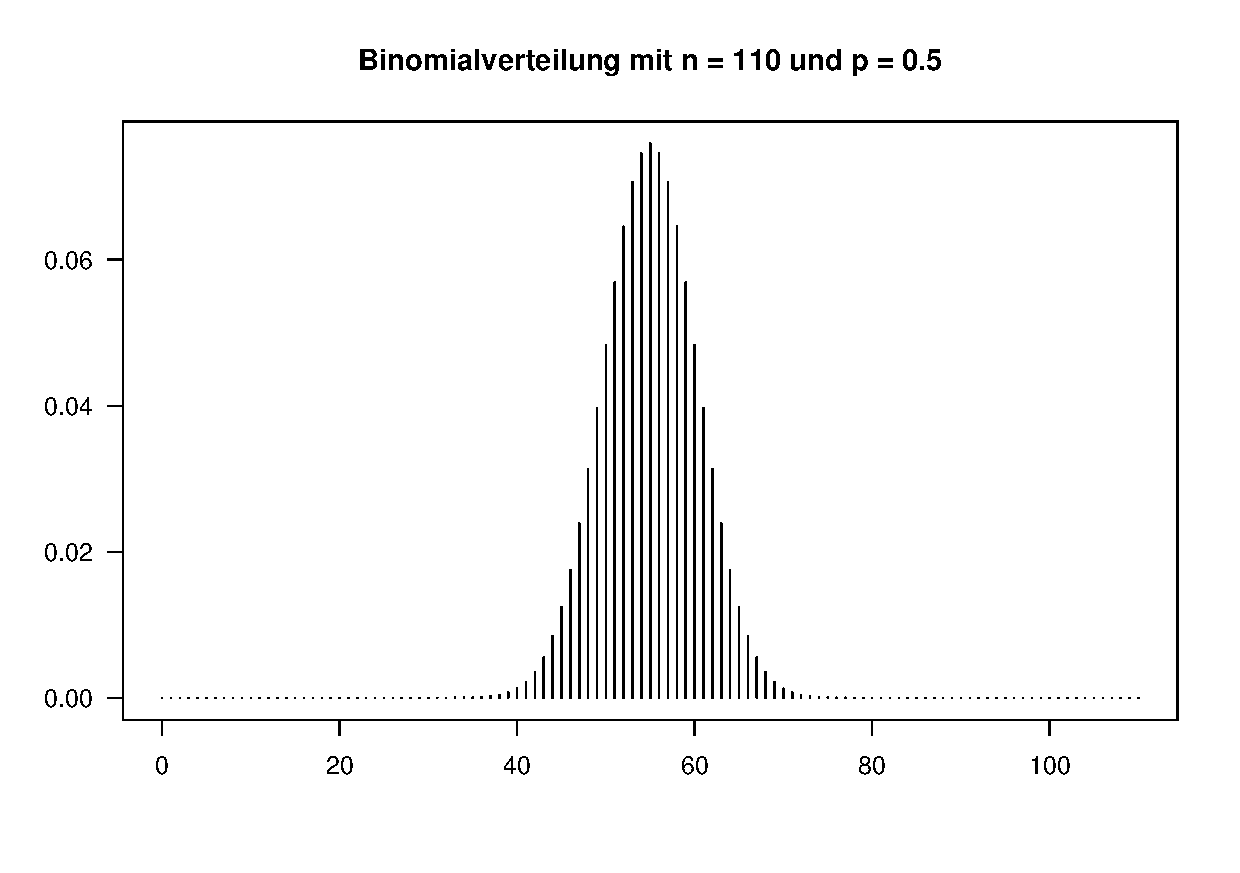
\includegraphics[scale=0.55]{binom.pdf}
	\end{center}
\end{frame}


\begin{frame}

\begin{block}{}
\begin{itemize}
\item[a)] Erfolgsanzahl entspricht dem Erwartungswert 
\end{itemize}
\end{block}
$$\mathbf{P}(X=55) = \binom{110}{55} \cdot 0,5^{55} \cdot 0,5^{110-55} = 0.0759$$

\pause

\begin{block}{}
\begin{itemize}
\item[b)] Erfolgsanzahl innerhalb des $2\sigma$-Intervalls $[ 44,52; 65,48]$
\end{itemize}
\end{block}
\begin{align*}
\mathbf{P}(44,52\leq X \leq 65,48) =  \mathbf{P}(X \leq 65) - \mathbf{P}(X \leq 44) \approx 0.9776- 0.0223= 0.9553 
\end{align*}

\pause

\begin{block}{}
\begin{itemize}
\item[c)] Erfolgsanzahl außerhalb des $2\sigma$-Intervalls  $[ 44,52; 65,48]$
\end{itemize}
\end{block}
$$1-\mathbf{P}(44,52\leq X \leq 65,48) = 1- 0.9553 = 0,0447$$


\end{frame}


\end{document}